
\chapter{Stretching our legs}

We've got a steep climb up ahead of us. What exactly are we up against? And
what will we see from the summit that will be worth all the effort to get
there?

As we did in the opening chapter of \textit{A Cool, Brisk Walk}, let's take the
two words of our subject -- ``Linear Algebra'' -- one at a time, and talk about
what they mean. And just like we did for ``Discrete Mathematics,'' we'll
consider the words in reverse order.

\section{``Algebra''}

\index{Algebra}
When most people hear the word ``algebra,'' they flash back to middle school,
to that subject where they first learned to work with letters (like $x$)
instead of just numbers (like 5) in a math class. They remember the quadratic
formula, collecting like terms, factoring expressions, and so on.

\index{algebra@``an algebra''}
That middle school class is indeed related to the subject of our book, but more
distantly than you might imagine. Properly speaking, that middle school subject
is a \textit{proper} noun: ``Algebra'' with a capital `A.' It's actually a
special case of the \textit{common} noun that mathematicians deal with: an
``algebra'' with a lower-case `a.' Okay. So what's ``\textit{an} algebra,''
then?

\index{object, mathematical}
\index{mathematical object}
An algebra is any system of mathematical objects together with operations that
can be used to combine them. The middle school Algebra is an example: the
``objects'' are numbers (or letters that stand for numbers) and the operations
are things like addition, multiplication, powers, roots, and the like. We can
take numbers (or stand-ins) like:

\vspace{-.25in}
\begin{align*}
5, x, 3, y, q, 17, 14, z, 9
\end{align*}

and combine them to build up a complex expression like:

\vspace{-.25in}
\begin{align*}
\frac{\frac{(5+x)^3}{y} - q\cdot 17}{\sqrt{(14+x)^z + 9+y}}.
\end{align*}

It looks kinda gross, but I think you'll agree that if you knew what numbers
each letter stood for, you could laboriously crank out the answer with a
calculator.

Another example was the algebra of sets we learned about in \textit{Cool, Brisk
Walk} chapter 2. We could take the sets $A, B, \mathbb{N},$ and $\mathbb{Q}$
and combine them with set operations to get:

\vspace{-.25in}
\begin{align*}
((A \cap \mathbb{N}) \cup \overline{B}) \times A - \overline{(\mathbb{Q} \cup
B)}.
\end{align*}

Or, from chapter 8 of \textit{Cool, Brisk Walk}, we could combine the logical
propositions $P, Q, R,$ and $S$ to get a compound proposition like:

\vspace{-.25in}
\begin{align*}
(\neg P \vee Q \wedge \neg (R \oplus P)) \Leftrightarrow (\neg S \Rightarrow P).
\end{align*}

Any system of mathematical objects and operations like this is an ``algebra.''
The subject of this book is \textit{linear} algebra in which the ``mathematical
objects,'' instead of being numbers or sets or propositions, are
\textbf{vectors} and \textbf{matrices}.

\subsection{Closure}
\index{closure}

Key to the notion of an algebra, by the way, is the notion of \textbf{closure}.
Closure means that when we combine two or more of the mathematical objects in
question, we get back another object \textit{of the same type.} For instance,
whether or not you can simplify $\frac{227}{45}$ in your head, you \textit{do}
know that when you divide 227 by 45 you will get \textit{a number}. Similarly,
if you take the union of two sets $D \cup M$, you will get \textit{a set}. And
if you take the exclusive-or of two propositions $L \oplus A$, you will get
\textit{a proposition}.

\index{porcupine}

This is important because without this guarantee, we couldn't build up complex
expressions and be certain they would mean anything. Take the expression $12 +
\frac{227}{45}$. Even without a calculator, you know these operations can in
principle be done, because whatever exact value $\frac{227}{45}$ turns out to
be, it's guaranteed to be \textit{a number}, and therefore it can be
meaningfully added to 12. If, when dividing one number by another, the result
might wind up being a \textit{set} (or a proposition, or a porcupine), then the
whole expression would become meaningless: you can't add a number to a
porcupine.

In this book we'll combine vectors and matrices in a myriad of different ways,
and we will always get vectors and matrices back. That's why they constitute
``an algebra.''

\section{``Linear''}

\index{linear}
\index{function}

The word \textit{linear} is related to the word \textit{line}: this is because
a function that is linear looks like a line when it's plotted. Suppose I make
\$11.75/hour at my part-time job, and I want to figure out my take-home pay for
last week's work. Obviously, my paycheck (before taxes and what-not) will be
11.75 times the number of hours I work. The left side of
Figure~\ref{fig:linearNLPlots} shows my hours vs.~my pay, which is, not
surprisingly, a line.

\begin{figure}[ht]
\centering
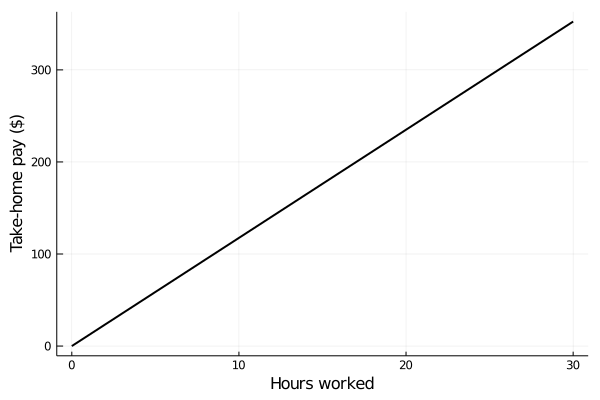
\includegraphics[width=0.45\textwidth]{linear.png}
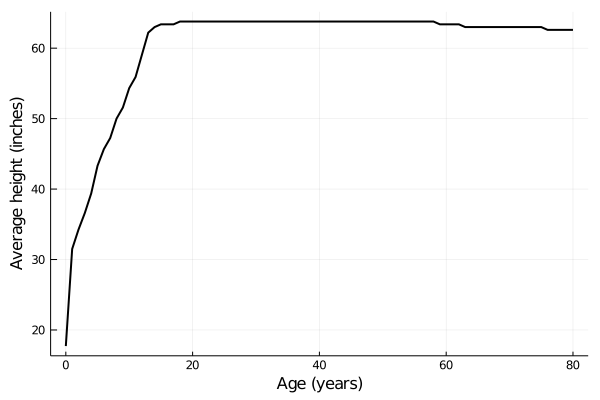
\includegraphics[width=0.45\textwidth]{nonlinear.png}
\caption{Linear and non-linear functions.}
\label{fig:linearNLPlots}
\end{figure}

By contrast, suppose I wanted to predict how tall a typical American human
female would be based on her age. While it's true that for most age ranges the
two variables increase together (just as more hours-worked implies more
take-home pay, so does more years-on-earth implies more inches-off-the-ground),
the plot is no longer a straight line (see the right side of
Figure~\ref{fig:linearNLPlots}).

